\Section{Ахо-Корасик и Укконен}{26 октября 2017}{Сергей Копелиович}

\Subsection{Бор}

\up
\hspace*{-0.8em}
\begin{tabular}{ll}
\vtop{\null\hbox{\parbox{12cm}{
Бор -- корневое дерево. Рёбра направлены от корня и подписаны буквами. 
Некоторые вершины бора подписаны, как конечные.

\down
Базовое применение бора -- хранение словаря \t{map<string, T>}.

\down
Пример из \href{https://en.wikipedia.org/wiki/Trie}{wiki} бора, содержащего словарь \\
\{A\,:\,15, to\,:\,7, tea\,:\,3, ted\,:\,4, ten\,:\,12, i\,:\,11, in\,:\,5, inn\,:\,9\}.

\down
Для строки \t{s} операции \t{add(s)}, \t{delete(s)}, \t{getValue(s)} \\
работают, как спуск вниз от корня.

}}}
&
\vtop{\null\hbox{\parbox{6cm}{
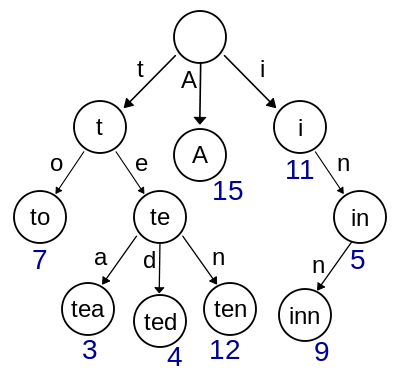
\includegraphics[width=5cm]{pics/trie.png}
}}}
\\
\end{tabular}

\down
Самый простой способ хранить бор: \t{vector<Vertex> t;}, где \t{struct Vertex \{ int id[$|\Sigma|$]; \}};\\
Сейчас рёбра из вершины \t{t} хранятся в массиве \t{t.id[]}. Есть другие структуры данных:
\begin{center}
	\begin{tabular}{lll}
		{\bf Способ хранения} & {\bf Время спуска по строке} & {\bf Память на ребро}\\
		\t{array} & $\O(|s|)$ & $\O(|\Sigma|)$ \\
		\t{list} & $\O(|s| \cdot |\Sigma|)$ & $\O(1)$ \\
		\t{map (TreeMap)} & $\O(|s| \cdot \log|\Sigma|)$ & $\O(1)$ \\
		\t{HashMap} & $\O(|s|)$ с большой const & $\O(1)$ \\
		\t{SplayMap} & $\O(|s| + \log S$ & $\O(1)$ \\
	\end{tabular}
\end{center}
Иногда для краткости мы будем хранить бор массивом \t{int next[N][$|\Sigma|$];}. \t{next[v][c] == 0} $\EQ$ ребра нет.

\THE{Сортировка строк}

Если мы храним рёбра в структуре, способной перебирать рёбра в лексикографическом порядке (не хеш-таблица, не список),
можно легко отсортировать массив строк: \\
($1$) добавить их все в бор, ($2$) обойти бор слева направо.\\
Для \t{SplayMap} и $n$ и строк суммарной длины $S$, получаем время $\O(S + n \log S)$.\\
Для \t{TreeMap} получаем $\O(S \log |\Sigma|)$.

\begin{Rem}
Если бы мы научились сортировать строки над произвольным алфавитом за $\O(|S|)$, то для $\Sigma = \Z$,
получилась бы сортировка целых чисел за $\O(|S|)$.
\end{Rem}

Часто размер алфавита считают $\O(1)$. \\
Например строчные латинские буквы -- $26$, или любимый для биологов $|\{A, C, G, T\}| = 4$.

\Subsection{Алгоритм Ахо-Корасика}

Даны текст $t$ и словарь $s_1, s_2, \dots, s_m$, нужно научиться искать словарные слова в тексте.

Простейший алгоритм, отлично работающий для коротких слов, -- сложить словарные слова в бор и
от каждой позиции текста $i$ попытаться пройти вперёд, откладывая суффикс $t_i$ вниз по бору, и отмечая все концы слов, которые мы проходим.
Время работы -- $\O(|t|\cdot\max|s_i|)$.

\down
Ту же асимптотику можно получить, сложив все хеши всех словарных слов в хеш-таблицу, и проверив, есть ли в хеш-таблице какие-нибудь подстроки
$t$ длины не более $\max|s_i|$.

\down
Давайте теперь соптимизируем первое решение также, как префикс-функция, позволяет простейший алгоритм поиска подстроки в строке улучшить до линейного 
времени. Обобщение префикс-функции на бор -- суффиксные ссылки:
\begin{Def}
$\forall$ вершины бора $v$:\\
$str[v]$ -- строка, написанная на пути от корня бора до $v$.\\
$suf[v]$ -- вершина бора, соответствующая самому длинному суффиксу $str[v]$ в боре.
\end{Def}

$\forall$ позиции текста $i$ насчитаем вершину бора $v_i \colon str[v_i]$ -- суффикс $t[0{:}i), |str[v_i]| \to \max$.

{\bf Пересчёт $v_i$:}
\begin{code}
v[0] = root, p = root
for (i = 0; i < |t|; i++)
	while (next[p][t[i]] == 0) // `нет ребра`
		p = suf[p]
	v[i + 1] = p = next[p][t[i]]
\end{code}
Чтобы цикл \t{while} всегда останавливался введём фиктивную вершину \t{f} и \\
сделаем \t{suf[root] = f, $\forall c$ next[f][c] = root}.

\down
{\bf Поиск словарных слов.} Пометим все вершины бора, посещённые в процессе: \t{used[v$_i$] = 1}. 
В конце алгоритма поднимем пометки вверх по суффиксным ссылкам: \t{used[v]} $\SO$ \t{used[suf[v]]}.
Для $i$-го словарного слова при добавлении мы запомнили вершину \t{end[i]}, тогда наличии этого слова в тексте лежит в \t{used[end[i]]}.
Также можно насчитывать число вхождений.

\down
{\bf Суффссылки.} Чтобы всё это счастье работало осталось насчитать суффссылки. 

\down
Способ \NO{1}: полный автомат. 
\begin{code}
suf[v] = go[suf[parent[v]]][parent_char[v]];
go[v][c] = (next[v][c] ? next[v][c] : next[suf[v]][c]);
\end{code}
Естественно, чтобы от \t{parent[v]} и \t{suf[v]} всё было уже посчитано, поэтому нужно или перебирать вершины в порядке bfs от корня, или считать эту динамику рекурсивно-лениво.

\down
Способ \NO{2}: пишем bfs от корня и пытаемся продолжить какой-нибудь суффикс отца.
\begin{code}
q <-- root
while q --> v:
	z = suf[parent[v]]
	while next[z][parent_char[v]] == 0:
		z = suf[z]
	suf[v] = next[z][parent_char[v]]
\end{code}
Этот способ экономнее по памяти, если \t{next} -- не массив, а, например, \t{map<int,int>}.
\begin{Thm}
Время построения линейно от длины суммарной строк, но не от размера бора.
\end{Thm}
\begin{proof}
Линейность от размера бора ломается на примере <<бамбук длины $n$ из букв $a$, из листа которого торчат рёбра по $n$ разным символам>>.
Линейность от суммарной длины строк следует из того, что если рассмотреть путь, соответствующий $\forall$ словарному слову $s_i$,
то при вычислении суффссылок от вершин именно этого пути, указатель $z$ в \t{while} всё время поднимался, а затем опускался 
не более чем на $1 \SO$ сделал не более $2|s_i|$ шагов.
\end{proof}

\pagebreak
\vspace*{-1.5em}
\Subsection{Суффиксное дерево, связь с массивом}

\up
\begin{Def}
Сжатый бор: разрешим на ребре писать не только букву, но и строку. 
При этом из каждой вершины по каждой букве выходит всё ещё не более одного ребра.
\end{Def}
\up\up
\begin{Def}
Суффиксное дерево -- сжатый бор построенный из суффиксов строки.
\end{Def}

\begin{Lm}
Сжатое суффиксное дерево содержит не более $2n$ вершин.
\end{Lm}
\begin{proof}
Индукция: база один суффикс, 2 вершины, добавляем суффиксы по одному, каждый порождает максимум \t{+}1 развилку и \t{+}1 лист.
\end{proof}

\up
\THE{Построение суффдерева из суффмассива\t{+}LCP}

Пусть мы уже построили дерево из первых $i$ суффиксов в порядке суффмассива.
Храним путь от корня до конца $i$-го. Чтобы добавить $(i+1)$-й, поднимаемся до высоты $LCP(i,i{+}1)$ и делаем новую развилку, новый лист.
Это несколько \t{pop}-ов и не более одного \t{push}-а. Итого $\O(n)$.

\THE{Построение суффмассива\t{+}LCP из суффдерева}

Считаем, что дерево построено от строки $s\$ \SO$ (листья \t{=} суффиксы).\\
Обходим дерево слева направо. Если в вершине используется неупорядоченный \t{map} для хранения рёбер, сперва отсортируем их.
При обходе выписываем номера листьев-суффиксов. \\
$LCP(i,i+1)$ -- максимально высокая вершина, из пройденных по пути из $i$ в $i+1$.\\
Время работы $\O(n)$ или $\O(n \log |\Sigma|)$.

\Subsection{Суффиксное дерево, решение задач}

\THE{Число различных подстрок.}

Это ровно суммарная длина всех рёбер. Так как любая подстрока есть префикс суффикса $\SO$ откладывается от корня дерева вниз до <<середины>> ребра.

\THE{Поиск подстрок в тексте.}

Строим суффдерево от текста. $\forall$ строку $s$ можно за $\O(|s|)$ искать в тексте спуском по дереву.

\THE{Общая подстрока $k$ строк.}

Построим дерево от $s_1\NO_1s_2\NO_2{\dots}s_k\NO_k$, найдём самую глубокую вершину, в поддереве которой
содержатся суффиксы $k$ различных типов. Время работы $\O(\sum |s_i|)$, оптимально по асимптотике.
Константу времени работы можно улучшать за счёт уменьшения памяти -- строить суффдерево не от конкатенации, а лишь от одной из строк.

\Subsection{Алгоритм Укконена}

Обозначение: $ST(s)$ -- суффиксное дерево строки $s$.\\
Алгоритм Укконена -- онлайн алгоритм построения суффиксного дерево.
Нам поступают по одной буквы $c_i$, мы хотим за амортизированное $\O(1)$ из $ST(s)$ получать $ST(sc_i)$.

\down
За квадрат это делать просто: храним позиции концов всех суффиксов, каждый из них продлеваем вниз на $c_i$, если
нужно, создаём при этом новые рёбра/вершины.

\down
Ускорение \NO{1}: суффиксы, ставшие листьями, растут весьма однообразно -- рассмотрим ребро $[l,r)$, 
за которое подвешен лист, тогда всегда происходит \t{r++}. Давайте сразу присвоим $[l,\infty)$.

\down
Теперь опишем жизненный цикл любого суффикса: \\
рождается в корне, ползёт вниз по дереву, разветвляется, становится саморастущим листом.

\pagebreak
\vspace*{-1em}
Нам интересно обработать только момент разветвления.

\begin{Lm}
$\LET$ Суффикс длины $k$ не разветвился $\SO$ все более короткие тоже не разветвились.
\end{Lm}
\begin{proof}
Суффикс длины $k$ не разветвился $\SO$ он встречался в $s$ как подстрока. \\
Все более короткие являются его суффиксами $\SO$
тоже встречаются в $s \SO$ не разветвятся.  
\end{proof}

Ускорение \NO{2}: давайте хранить только позицию самого длинного неразветвившегося суффикса.
Пока он спускается по дереву, ничего не нужно делать. Как только он разветвится, нужно научиться быстро переходить к следующему по длине 
(отрезать первую букву).

\down
Ускорение \NO{3}: отрезать первую букву \t{=} перейти по суффссылке, давайте от всех вершин поддерживать суффссылки.
Если мы были в вершине, когда не смогли пойти вниз, теперь всё просто, перейдём по её суффссылке.
Если же мы стояли посередине ребра и создали новую вершину $v$, от неё следует посчитать суффссылку. 
Для этого возьмём суффссылку её отца $p[v]$ и из $suf[p[v]]$ спустимся вниз на строку, соединяющую $p[v]$ и $v$.

\begin{code}
void build( char *s ) {
	int N = strlen(s), VN = 2 * Ns;
	int vn = 2, v = 1, pos; // `идём по ребру из p[v] в v, сейчас стоим в pos`
	int suf[VN], l[VN], r[VN], p[VN]; // `<<ребро p[v] $\to$ v>> = s[l[v]:r[v])`
	map<char,int> t[VN]; // `собственно рёбра нашего бора`
	for (int i = 0; i < `\blue{$|\Sigma|$}`; i++) t[0][i] = 1; // `0 = фиктивная, 1 = корень`
	l[1] = -1, r[1] = 0, suf[1] = 0;
	for (int n = 0; n < N; n++) {
		char c = s[n];
		auto new_leaf = [&]( int v ) {
			p[vn] = v, l[vn] = n, r[vn] = `\blue{$\infty$}`, t[v][c] = vn++;
		};
		go:;
		if (r[v] <= pos) { // `дошли до вершины, конца ребра`
			if (!t[v].count(c)) { // `по символу $c$ нет ребра вперёд, создаём`
				new_leaf(v), v = suf[v], pos = r[v];
				goto go;
			}
			v = t[v][c], pos = l[v] + 1; // `начинаем идти по новому ребру`
		} else if (c == s[pos]) {
			pos++; // `спускаемся по ребру`
		} else {
			int x = vn++; // `создаём развилку`
			l[x] = l[v], r[x] = pos, l[v] = pos;
			p[x] = p[v], p[v] = x;
			t[p[x]][s[l[x]]] = x, t[x][s[pos]] = v;
			new_leaf(x);
			v = suf[p[x]], pos = l[x]; // `вычисляем позицию следующего суффикса`
			while (pos < r[x])
				v = t[v][s[pos]], pos += r[v] - l[v];
			suf[x] = (pos == r[x] ? v : vn);
			pos = r[v] - (pos - r[x]);
			goto go;
		}
	}
}
\end{code}

\pagebreak
\vspace*{-1.5em}
\begin{Thm}
Суммарное время работы $n$ первых шагов равно $\O(n)$.
\end{Thm}
\begin{proof}
Понаблюдаем за величиной $\PHI$ ``число вершин на пути от корня до нас''.\\
Пока мы идём вниз, $\PHI$ растёт, когда переходим по суффссылке, $\PHI$ уменьшается максимум на $1$
$\SO$ суммарное число шагов вниз не больше $n$.
\end{proof}

\up
\Subsection{LZSS}

Решим ещё одну задачу -- сжатие текста алгоритмом LZSS.

В отличии от использования массива, дерево даёт чисто линейную асимптотику и простейшую реализацию --
насчитаем для каждой вершины $l[v] =$ самый левый суффикс в поддереве и при попытки найти $j < i \colon LCP(j, i) = \max$ будем
спускаться из корня, пока $l[v] < i$.
